\documentclass[12pt]{article}
\usepackage[utf8]{inputenc}
\usepackage[T1]{fontenc}
\usepackage[spanish,es-lcroman]{babel}
\usepackage{amsmath}
\usepackage{amsthm}
\usepackage{physics}
\usepackage{tikz}
\usepackage{float}
\usepackage{cancel}
\usepackage[autostyle,spanish=mexican]{csquotes}
\usepackage[per-mode=symbol]{siunitx}
\usepackage{gensymb}
\usepackage{multicol}
\usepackage{enumitem}
\usepackage{stackengine}
\usepackage{stix}
\usepackage[left=2.00cm, right=2.00cm, top=2.00cm, 
     bottom=2.00cm]{geometry}

\usepackage{Estilos/ColoresLatex}
\usepackage{makecell}
\usepackage{wrapfig}
% \usepackage{titlesec}
\usetikzlibrary{angles,quotes}
\newcommand{\sectionbreak}{\clearpage}

\newcommand{\textocolor}[2]{\textbf{\textcolor{#1}{#2}}}
%\renewcommand{\questionlabel}{\thequestion)}

\newcommand{\Cancel}[2][black]{{\color{#1}\cancel{\color{black}#2}}}

\newcommand\deci[1]{%
    \kern-.4ex\stackunder[0.4pt]{$#1$}{$\color{blue}\acwunderarcarrow$}
}

\newcommand\decposl[1]{%    <--- Decimal position to left
    \kern-.4ex\stackunder[0.4pt]{$#1$}{%
      \reflectbox{$\color{red}\kern-.6ex\acwunderarcarrow$}
      }
}

\decimalpoint
\sisetup{bracket-numbers = false}

\title{\vspace*{-2cm} Superconductividad}
\author{M. en C. Ramón Gustavo Contreras Mayén \\ {\fontsize{14}{14}\selectfont Universidad del Valle de México. Campus San Rafael}}
% \institute{Universidad del Valle de México. Campus San Rafael.}
\date{}

\begin{document}
\maketitle

\section{Resistencia de materiales.}

\subsection{Resistencia y conductividad.}

La resistencia eléctrica y la conductividad eléctrica son dos conceptos fundamentales en la teoría de la electricidad. Ya que describen la capacidad de un material para oponerse o permitir el flujo de corriente eléctrica a través de él.

\subsection{Resistencia eléctrica.}

La resistencia eléctrica, representada por la letra $R$, es una medida de la oposición que ofrece un material al flujo de corriente eléctrica.  Se define como la relación entre la diferencia de potencial (voltaje) aplicada a través de un material y la corriente eléctrica que fluye a través de él.

Según la ley de Ohm:
\begin{align*}
R = \dfrac{V}{I}
\end{align*}
donde $V$ es el voltaje aplicado e $I$ es la corriente eléctrica.

La unidad de resistencia en el Sistema Internacional (SI) es el Ohm (\unit{\ohm}).

\subsection{Conductividad eléctrica.}

La conductividad eléctrica, representada por la letra $\sigma$ (sigma), es la medida de la facilidad con la que un material permite el flujo de corriente eléctrica a través de él.

Se define como el inverso de la resistividad eléctrica $(\rho)$ del material:
\begin{align*}
\sigma = \dfrac{1}{\rho}
\end{align*}
La resistividad $(\rho)$ es una medida de la capacidad de un material para oponerse al flujo de corriente eléctrica.

La unidad de conductividad eléctrica en el SI es el siemens por metro (S/m).

\subsection*{Relación entre $\sigma$ y $\rho$}

Cuanto mayor sea la conductividad eléctrica de un material, menor será su resistividad y viceversa. Los materiales conductores, como los metales, tienen alta conductividad y baja resistencia, mientras que los materiales aislantes tienen baja conductividad y alta resistencia.


% \subsection{Relación entre resistencia y conductividad}


% Relación entre $R$ y $\sigma$}
% Hay una relación inversa entre resistencia y conductividad: cuanto mayor sea la resistencia eléctrica de un material, menor será su conductividad, y viceversa.


% Relación entre $R$ y $\sigma$}
% Esta relación se puede expresar matemáticamente como:

% \begin{align*}
% R =\dfrac{1}{\sigma \cdot A}
% \end{align*}
% donde \enquote{R} es la resistencia, \enquote{$\sigma$} es la conductividad, y \enquote{A} es el área de la sección transversal del material a través del cual fluye la corriente eléctrica.


% Relación entre $R$ y $\sigma$}
% Los materiales conductores, como los metales, tienen alta conductividad y baja resistencia, mientras que los materiales aislantes tienen baja conductividad y alta resistencia.


% Relación entre $R$ y $\sigma$}
% La resistencia eléctrica y la conductividad eléctrica son dos conceptos complementarios que describen la capacidad de un material para permitir o resistir el flujo de corriente eléctrica.


% Relación entre $R$ y $\sigma$}
% La conductividad es una medida de lo bueno que es un material para conducir la electricidad, mientras que la resistencia es una medida de su oposición al flujo de corriente.


\section{Superconductividad.}

\subsection{Definición.}

La superconductividad es un fenómeno físico que se produce en ciertos materiales a temperaturas muy bajas Generalmente por debajo de una temperatura crítica específica. Existen superconductores convencionales, en donde la temperatura crítica es relativamente baja, variando desde unos \SI{9}{\kelvin} hasta \SI{18}{\kelvin}, y también se encuentran los superconductores de alta temperatura, que tienen temperaturas críticas mucho más altas, que van desde unos \SI{30}{\kelvin} hasta \SI{138}{\kelvin}.

El reto tecnológico en esta área de la física, es lograr materiales superconductores en temperaturas ambiente, es decir, sin que haya una necesidad de contar con sistemas que enfríen el material, ya que la ganancia energética de alguna manera no está compensada: lo que se puede obtener como beneficio del material superconductor, se requiere invertir en energía para enfriarlo.

Donde estos materiales exhiben:
\begin{enumerate}
\item Una resistencia eléctrica cero.

Uno de los aspectos más destacados de la superconductividad es que los materiales superconductores tienen una resistencia eléctrica cero cuando se enfrían por debajo de su temperatura crítica. Esto significa que pueden transportar corriente eléctrica sin pérdida de energía.
\item Expulsan completamente el campo magnético aplicado (efecto Meissner-Ochsenfeld).

Los superconductores expulsan completamente el campo magnético aplicado en su interior cuando se encuentran en el estado superconductor, lo que se conoce como el efecto Meissner-Ochsenfeld. Esto implica que los superconductores son diamagnéticos (repelen el campo magnético) perfectos en estado superconductor.
\end{enumerate}

Este fenómeno fue descubierto por primera vez en 1911 por los físicos holandeses Heike Kamerlingh Onnes y Gilles Holst cuando estudiaban las propiedades eléctricas de ciertos metales a temperaturas extremadamente bajas.

\subsection{Transición a estado superconductor.}

En la siguiente gráfica se comparan dos materiales, uno de ellos normal, en donde se aprecia que mientras se enfría su valor de resistencia disminuye, hecho que se explica con un poco más de física moderna, pero llegará a un valor de resistencia determinado, es decir, no bajará a cero su valor de resistencia. Mientras que otro material llamado superconductor, en un primer momento presenta resistencia eléctrica interna, pero al llegar al valor de temperatura crítica $T_{C}$, de manera súbita, su valor de resistencia interna se hace cero, mientras siga por debajo de la $T_{C}$ permanecerá en ese estado.
\begin{figure}[H]
    \centering
    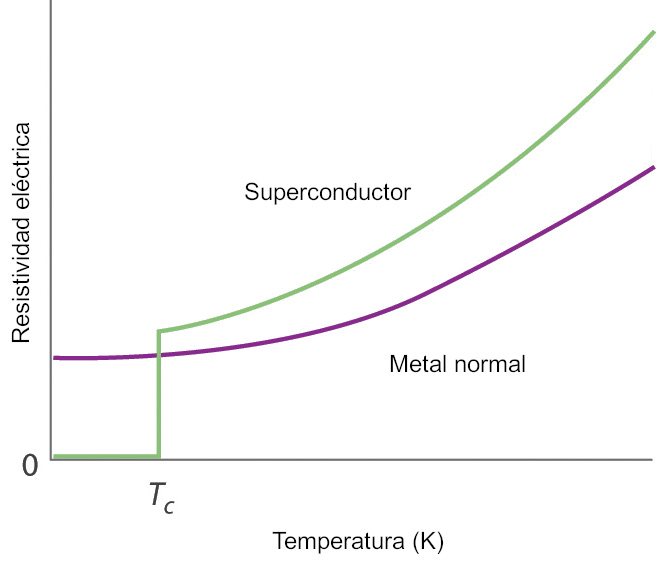
\includegraphics[scale=1.5]{Imagenes/Superconductividad_01.jpg}
\end{figure}
Si el material supeconductor supera la $T_{C}$ pierde sus propiedades de superconductor y regresa a un estado normal, es decir, con resistencia interna. 

\subsection{Aplicaciones.}

La superconductividad tiene numerosas aplicaciones tecnológicas:

\begin{enumerate}
\item Creación de imanes superconductores para la resonancia magnética nuclear (RMN) y la resonancia magnética (RM) en medicina.
\item Transmisión de energía eléctrica sin pérdidas.
\item Aceleradores de partículas.
\item Fabricación de dispositivos electrónicos de alta sensibilidad, como detectores de radiación.
\end{enumerate}

En la siguiente figura se muestra el efecto de levitación magnética, conocido como efecto Meissner.
\begin{figure}[H]
    \centering
    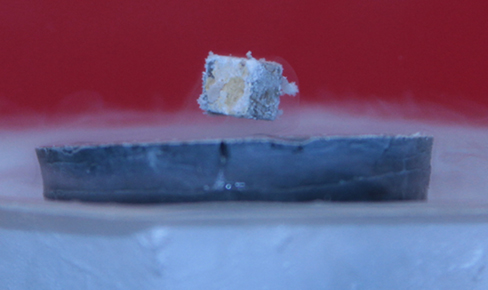
\includegraphics[scale=1.5]{Imagenes/Superconductividad_02.jpg}
\end{figure}

\end{document}
